\chapter{FAS系统设计}
接下来的部分将包括FAS系统简单介绍。通过综合考虑这些因素,我们将确保FAS系统能够在城市轨道交通运营中发挥重要作用,保障乘客和工作人员的生命安全。车站级火灾自动报警系统如\ref{fig:车站级火灾自动报警系统}所示。
% TODO: \usepackage{graphicx} required
\begin{figure}[h]
	\centering
	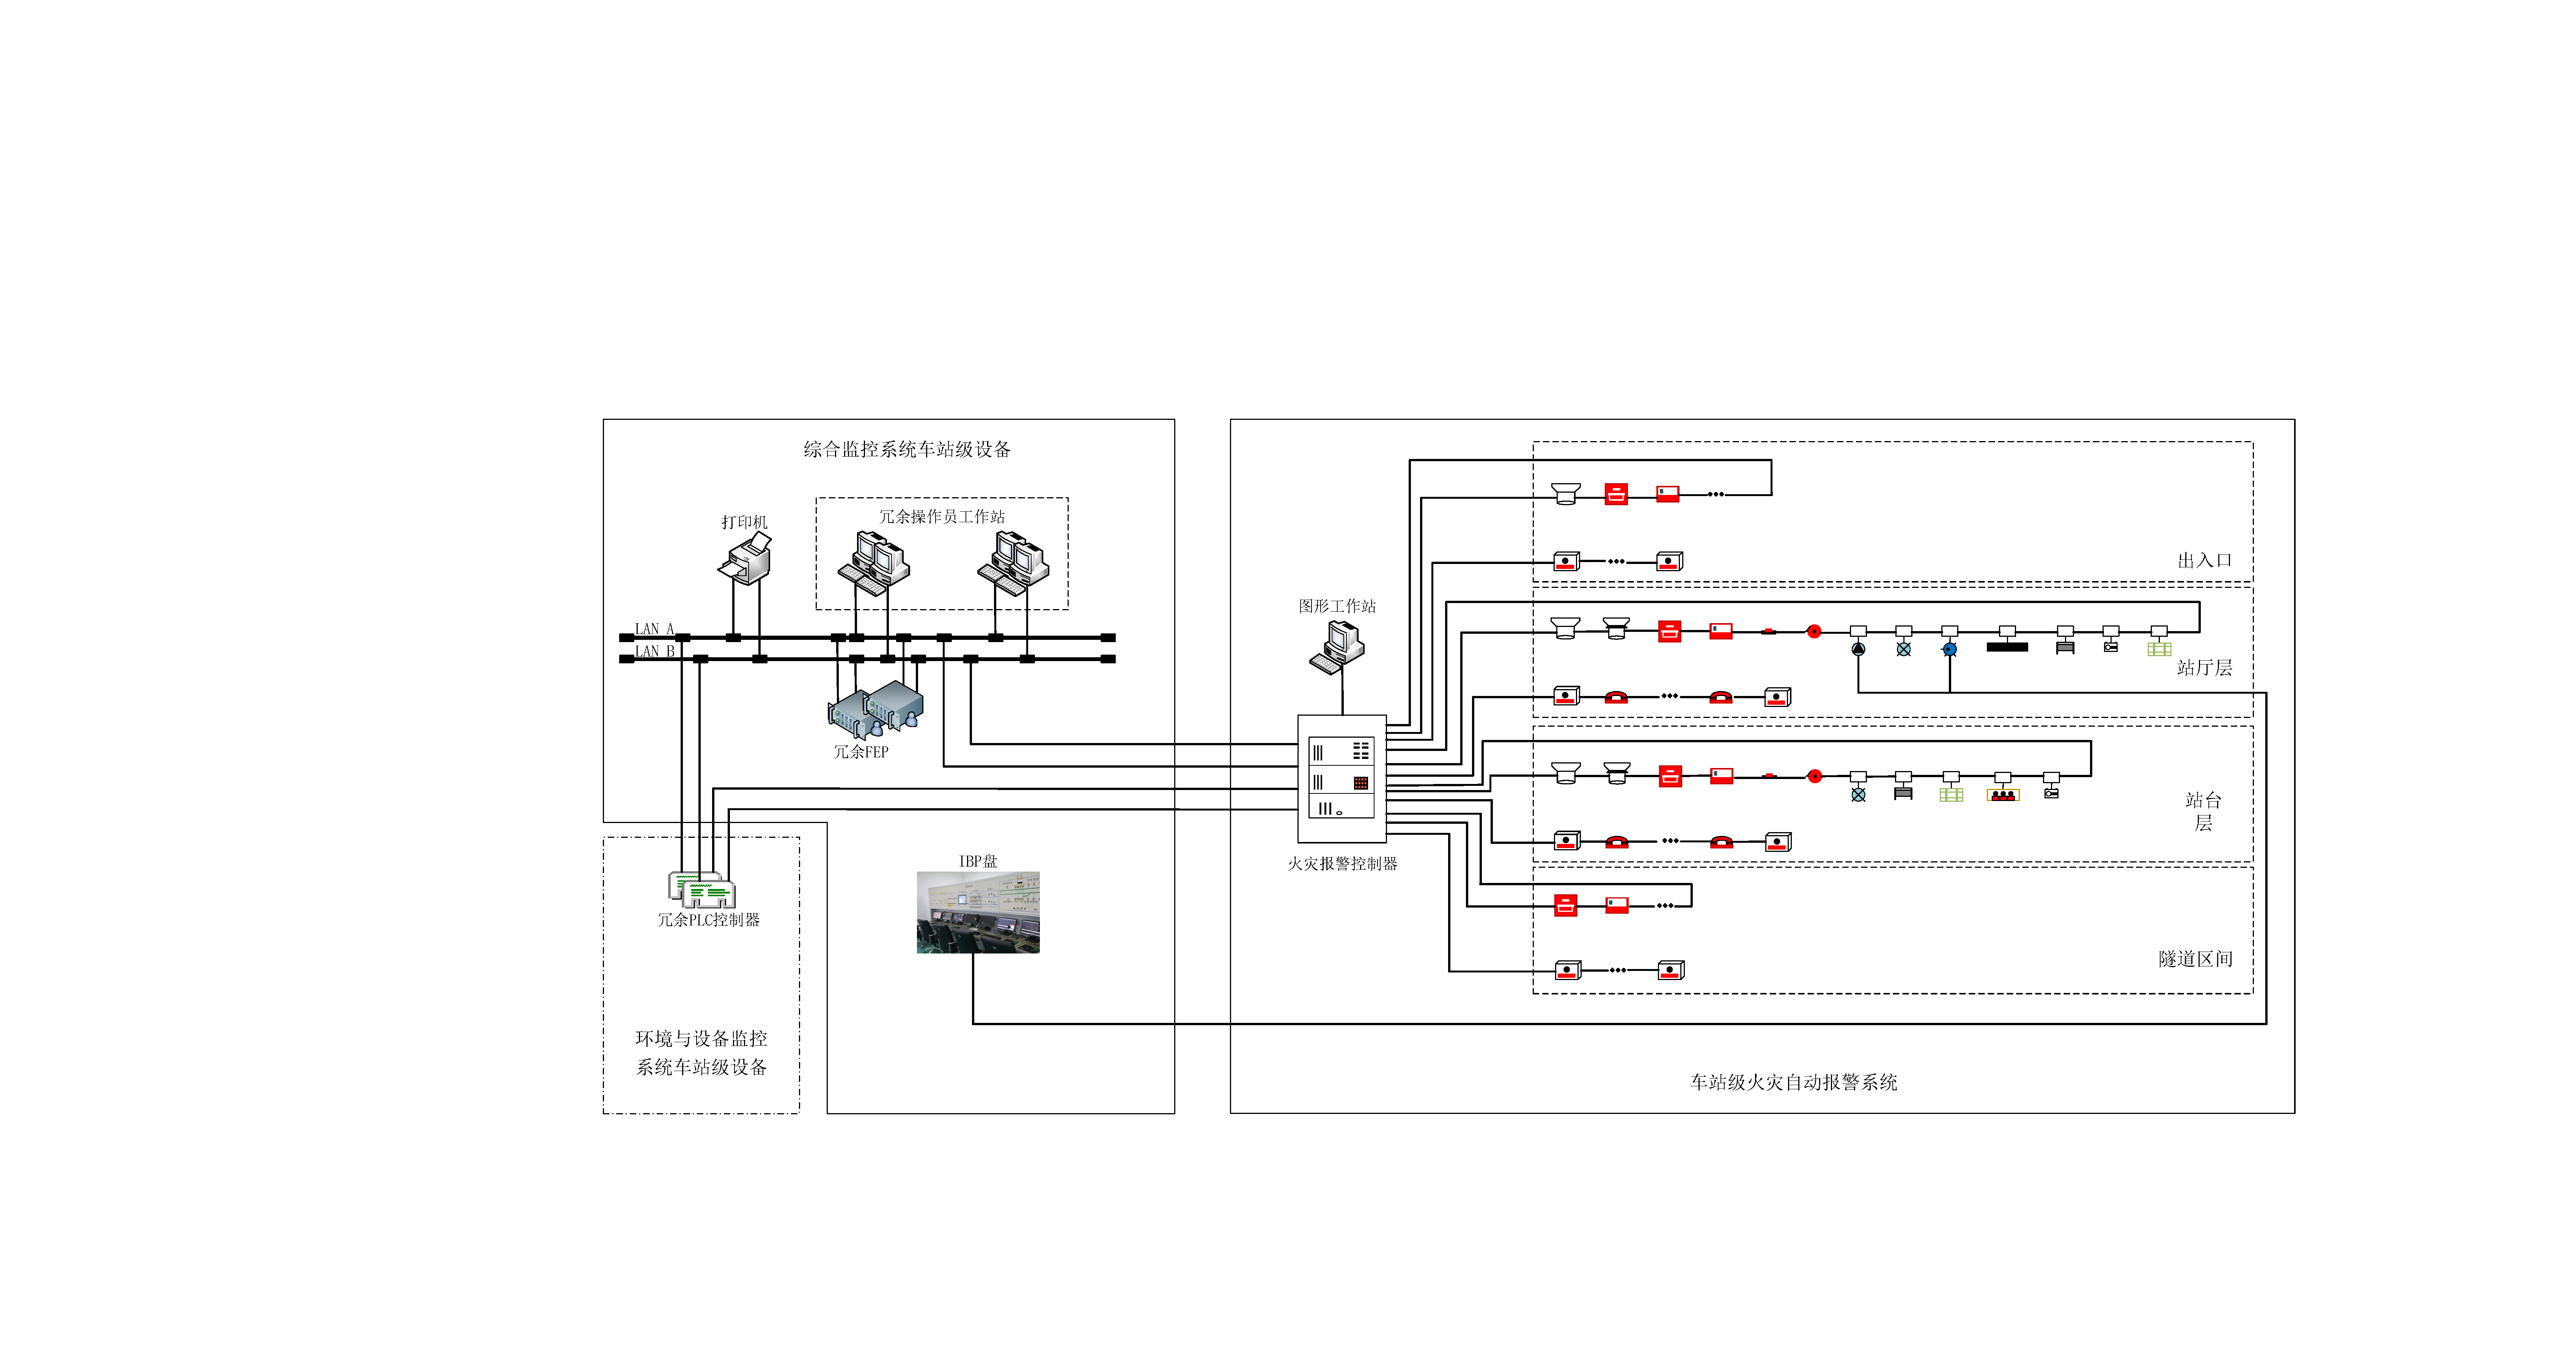
\includegraphics[width=0.8\linewidth]{figures/车站级火灾自动报警系统}
	\caption{车站级火灾自动报警系统}
	\label{fig:车站级火灾自动报警系统}
\end{figure}

\section{火灾自动报警系统应用分析}
作为 FAS(Fire Alarm System,火灾自动报警系统)系统运营维护单位,应该对该系统技术方案有全面深入的了解,对设备运行及设置的不合理点有清楚的掌控,才能做到提前预控,降低设备运行风险,提高系统稳定性。而 FAS 系统作为消防控制专业系统,技术设置方案是否合理,能否保证运行稳定,和其自身发生故障会否影响其监控设备单元的正常运行,都是要仔细考虑的内容,因此有必要仔细分析技术方案中的潜在不合理点,避免因技术方案缺陷而影响车站消防报警系统的正常运行。
\section{火灾自动报警功能}
综合监控系统应实现集成子系统FAS的中央级和车站级全部功能,对车站、车辆段、 区间所、区间等进行系统的、全面的、有效的火警探测及消防设备的监控管理。涉及报 警确认、控制指令下发等功能在设计联络阶段最终确定。综合监控系统具体实现功能如 下:
\subsection{中央级功能}
对地铁车站内的消防通风设备、消防泵设备、非消防电源设备等车站设备、地铁空 间,进行系统的、全面的、有效的火灾情况的监控及管理;采集、处理火灾报警信息, 进行历史资料档案。保证在列车火灾事故状态下,更好地协调车站设备的运行,充分发 挥各种设备应有的作用,保证乘客的安全和财产的损失。中央级保留与天津市公安消防 局消防控制中心联网的功能。\par 
综合监控系统中央级作为全线FAS的调度、管理中心,对全线报警系统信息及消防 设施有监视、控制及管理权,对车站级的防救灾工作有指挥权。通过全线防灾直通电话、 闭路电视、列车无线电话等通信工具,组织指挥全线防救灾工作。\par 
编制、下达全线FAS运行模式,火灾时确定全线火灾自动报警系统的运行模式,监 视运行工况。应能够完成对全线所有车站火灾报警控制器、GCC的程序修改并通过网络远程下载。\par 
接收各车站级报送的火灾报警信息和FAS监控设备的运行状态及故障信息,并记录 存档,按信息类别进行历史资料档案管理。\par
中央级通过车站级接收报警设备信息,向火灾区间相关车站下达模式控制指令,相关车站执行救灾模式。\par
在地下区间发生火灾时,综合监控系统中央级对火灾点相关车站发布救灾运行模式的控制指令。\par
接收列车无线电话报警,当列车在区间发生火灾事故时,对车站级发布、实施灾害工况指令,将相应救灾设施转为按预定的灾害模式运行。\par
当单水源车站发生火灾时,若本站水源故障,通过中央级启动备用车站消防水系统。\par
中央级不仅能够通过网络,实现对网络上的节点设备的管理、监视和控制,还必须实现对各个车站级的火灾报警控制器、气体灭火控制器、GCC及车站、区间、车辆段火灾报警设备等的工作状态进行监视。\par
中央级能够自动监测与相关系统的数字接口状态,及时报告接口故障和故障类型。\par
中央级应满足高可靠的要求,确保运营安全。\par
由于本工程换乘车站较多,火灾时本工程控制中心综合监控系统发送和接受有关火 灾信息,同时预留将其发送给其它相关地铁线路的控制中心调度系统的功能。

管理功能:

(1)全线火灾模式表管理。根据地铁火灾地点的不同,对火灾模式表进行下发。所有的操作过程记入事件日志。\par 
(2)系统运行参数管理
中央级综合监控系统能实现对系统设备的参数化管理功能,通过参数设置来确定系 统运行与监控方案,例如:探测器的隔离、探测器灵敏度的调整等设置。参数设置修改完毕后,通过网络下载到各车站的报警控制器中。\par 
(3)监督火灾模式运行工况中央级可监视火灾联动模式设备的运行工况,监视各站点(含区间)消防设备的正 常运行、报警及故障信息。\par 
(4)确定系统运行工况。在区间发生火灾情况下,按照发生火灾的不同地点启动火灾联动模式,由于区间发 生火灾涉及到相邻多个站,由中央级操作人员手动下发火灾联动模式。在车站火灾情况下,中央级具备监视功能,由车站下发火灾模式,当火灾发生漫延时,中央级进行指挥协调相关车站及系统投入进行救灾。\par 
(5)设备状态信息的处理。中央级能够接受各车站报送的设备运行状态、设备故障报警信息、系统参数监测数 据并能完成数据处理、做历史资料存档的管理。\par 
(6)指挥管理功能。通过全线防灾调度电话、闭路电视、列车无线电话等通信工具,组织、指挥、管理 全线防救灾工作。

监视功能:

(1)分区域设备状态。车站平面图是分区域显示。选择不同的区域按钮,显示相应区域平面图;如分别显示站台、换乘厅、车站公共区、设备管理用房、区间等区域画面。\par
(2)车站系统图分系统显示。选择不同的系统按钮,显示各系统图:如分别显示FAS图、动力照明系统图、电缆 夹层及区间实时温度曲线图。\par
(3)控制方式显示。在中央级和车站级工作站每个监控界面都能显示系统或设备的当前控制权,以体现 控制优先级。\par
(4)系统显示。在全线线路概貌图中用不同的颜色反映各车站及区间不同的火灾工况。某个车站或某区间运行在火灾工况下,在中央级工作站显示界面上可自动弹出火灾 报警信息,并通过画面颜色和报警提示显示火灾工况。

控制功能:

(1)单点控制。中央级环调监控功能界面具有设备的远程控制功能,可对单个设备(区间设备)进 行单设备控制。\par
(2)模式号控制。中央级具有模式号控制功能,可向车站报警控制器发送控制命令,报警控制器将进行优先级和冲突判断,根据判断结果运行控制命令对设备进行控制。
\subsection{车站级功能}
车站级能够接受中央级下达的各种监控指令与火灾模式控制指令,并下传到车站火 灾自动报警控制器,执行中央级制定的运行方案。车站级实现管辖范围内设备的自动监视与控制、重要设备的手动控制。车站级能够实现管辖范围内实时火灾的报警功能,监视管辖范围内的火情,自动化 管理火灾自动报警系统及防救灾设备,控制防救灾设施,显示运行状态,将所有信息上 传至中央级。接收中央级指令或独立组织、管理、指挥管辖范围内防救灾工作。向本站BAS发布确认的火灾信息,同时控制专用防排烟设备、消防泵等救灾设备进 入救灾模式运行。

监视功能

(1)设备动态图形显示功能。操作员通过平面图、系统图等人机界面可以直观地看到设备当前的工作状态,还可 看到设备的运行效果。通过鼠标的单击可以弹出设备属性框,看到具体的设备属性信息 和完成基本操作。\par
(2)故障报警功能。实时、可靠的报警系统可以使用户快速区分和辨别故障,减少系统的故障时间。\par
(3)数据查询。操作员在报警控制器上通过报警查询、事件查询功能可以方便地完成历史数据查 询、打印等工作。\par
(4)监视车站管辖范围内(含区间)灾情,采集火灾信息。\par
(5)自动弹出火灾报警信息并显示报警点,显示防救灾设施运行状态及所在位置画 面。\par
(6)监视消防泵的启、停、故障状态信号、水泵吸水管的压力报警值、水泵扬水管 的压力报警值、消防泵自巡检信号。\par
(7)监视本系统供电电源的运行状态。\par
(8)监视车站所有专用消防设备的工作状态。

控制功能:

根据火灾发生位置及火灾联动模式要求,按预先编制好的控制程序向车站的专用消 防设备,根据选定的控制方式发布救灾指令(包括但不限于):单点控制:车站级综合监控系统的监控功能界面具有设备的远程控制功能,可对单 个设备(区间设备)进行单设备控制。模式号控制:属于一种特定的设备组控制。模式的定义是根据工艺设计要求而形成, 其触发可有两种方式:人为触发和自动触发。

显示功能:

此功能与中央级系统的多级显示功能相同。每个监控画面都集工艺系统状态、设备状态、报警、控制等多种功能于一身,包含 显示和操作能力。\par
(1)分区域设备状态。车站平面图是分区域显示的。选择不同的区域按钮,显示相应区域平面图,如分别 显示站台、车站公共区、附属用房等画面。车站系统图是分系统显示的,选择不同的系统按钮,显示各系统图,如分别显示事 故电源系统图、消防通风系统图、消防给排水系统图、电扶梯系统。\par
(2)控制方式显示在车站级工作站每个监控界面都能显示系统或设备的当前控制权,以体现控制优先 级。

系统对时功能:

综合监控系统向FAS系统火灾报警控制器和GCC提供的网络时钟信号,统一FAS系 统内部的各个设备的时间,站间时钟信号相差不大于15ms。

\section{FAS 系统与 BAS 系统接口的稳定性分析}
地铁 FAS 系统进行火灾的探测、确认及报警,并向 BAS(Building Automation System,环境与设备监控系统)的 PLC 发送相应火灾模式指令,联动 BAS 执行火灾运行模式;同时接收BAS 反馈的模式执行状态信息[3]。BAS 系统接收 FAS 发送来的火灾模式信息后按既定原则执行火灾运行模式,实现关联设备的运行,并向 FAS 反馈模式执行状态信息[4]。地铁某线路 FAS 系统与 BAS 系统的通信接口设置在车站综控室的 IBP 盘(Inte原grated Backup Panel,综合后备盘)专用 PLC 上,通过双绞线连接车站火灾报警控制器与 PLC串口通信模块,实现 FAS 系统与BAS 系统间的信息互传功能,使两系统可以配合或独立实现对车站消防设备的联动控制。\par 
(1)分析:此方案中将 FAS 与 BAS 专业的通信接口采用单通道通信,如 PLC CPU死机或火灾报警器通信网卡损坏,则没有备用的硬件可以切换,导致与 FAS 通信立即中断。故目前方案对于 FAS 与 BAS 之间通信的保障力度不足。\par 
(2)改进措施:对于 FAS 专业,首先应该配置双通道冗余通信,互为备用,不应借助 IBP 盘的 PLC 转接,应该直接连接至车站主端车站级 PLC 上,可直接在 PLC 上添加两套互为备用的串口通信模块,直接与 FAS 进行通信。如要更进一步提高通信可靠性,可以对与FAS通信的接口设置较高级别的报警提示,如通信中断设置为 2 级报警(仅次于火灾报警级别),及时提醒维修人员对于通信故障进行修复。

\begin{figure}[h]
	\centering
	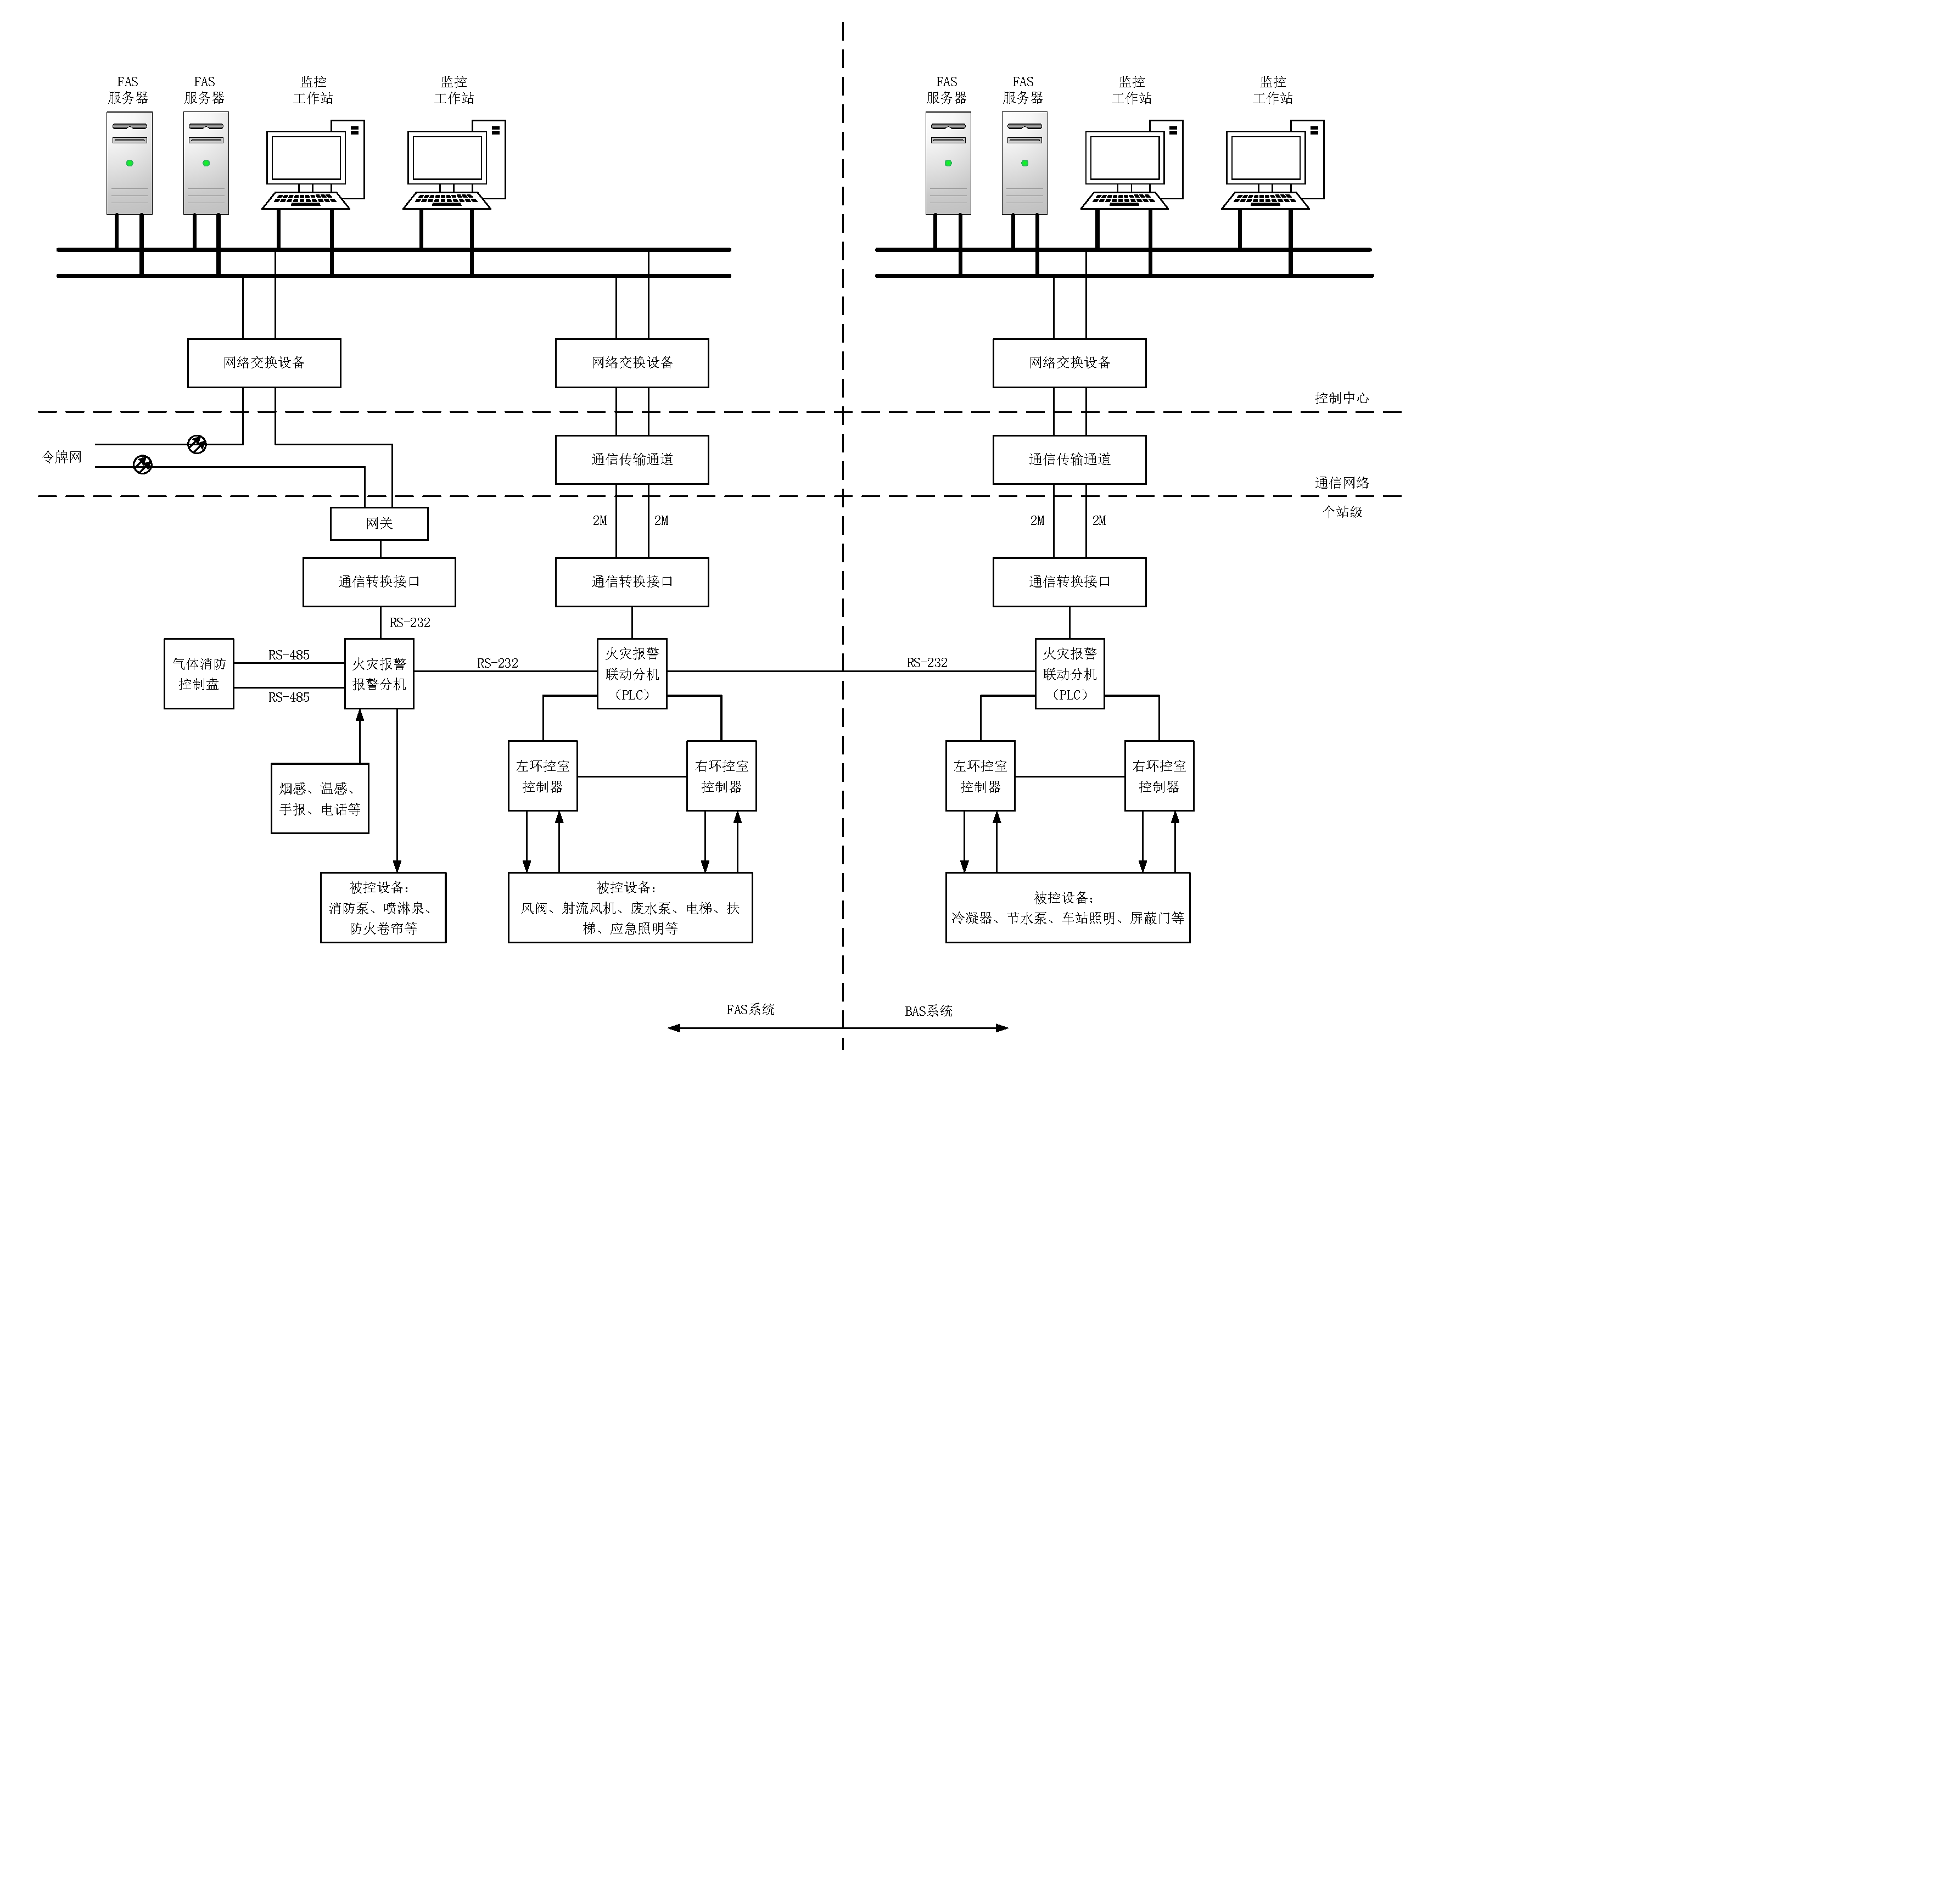
\includegraphics[width=1.0\textwidth]{FAS与BAS联动示意图.pdf}
	\caption{FAS与BAS联动示意图}
	\label{FAS与BAS联动示意图}
\end{figure}

\section{消防联动功能的应用性分析}
考虑到在车站发生火灾的情况下,BAS 的各种通信网络极有可能被火势所损坏,此时如不能对排烟风机进行控制,将影响消防排烟功能,故按照地铁的设计规范要求,BAS 系统在综控室设置一套 IBP 盘,将部分消防设备(消防泵、走廊专用排烟风机)采用硬线接口直接连接到消防设备的控制箱上,在 IBP 盘可完成紧急情况下有关的消防设备手动控制的功能。而车站大风机、管理用房排风机等设备的应急启动则通过 IBP 盘上设置的一个触摸屏集成控制。\par 
(1)分析:该线路车站 IBP 盘触摸屏集成控制车站大风机等进行火灾模式下发,BAS 系统模式执行反馈时间设置为 60 s,但由于风机联锁风阀的动作响应时间不同,联锁风阀在 60 s 内如未正常开启,则会造成车站风机不启动、模式下发失败等问题,影响发生火灾时车站排烟系统正常联动。另 IBP 盘上设置的气灭急停按钮是利用硬线连接继电器后接入气灭系统启动电气回路中,按下急停按钮,直接作用继电器断开电气回路,从而达到停止气灭系统启动的原理,但一旦按下 IBP 盘上气灭急停按钮,电气回路继续接通,气灭系统继续进行启动。此时如现场信号未进行复位撤销,仍会造成勿喷。\par 
(2)改进措施:针对风机与联锁风阀动作时间不同问题,可在 BAS 模式启动模式程序中增加延时启动命令,先执行相关联锁风阀启动,启动成功后,风机收到启动成功反馈信息后再进行风机等联动模式启动。或把火灾模式下发命令改为常保持信号下发,直到动作完成后,返回信号,终止命令。这样可以消除因风机联锁风阀响应时间造成的风机不能正常启动问题。另外地铁车站主风机设计为送、排两用风机,不同火灾模式下执行的功能不同,为避免风机正、反转无间隔切换造成电机制动过热的情况发生,在风机正、反转切换程序中加入收到反馈信号延时启动功能,对风机起到保护,提高火灾模式下排烟工况成功率。\par 
IBP 盘气灭急停按钮可采用带蜂鸣功能的按钮,同时在 IBP盘直接控制继电器的常开点处接入蜂鸣器,只要触发 IBP 盘紧急停止按钮,该继电器常开点闭合,蜂鸣器鸣响。紧急止喷时在综控室与现场双重蜂鸣器提示下,可提高综控室值守人员与现场人员的警惕性,降低 IBP 盘急停按钮按起而现场未复位所产生的二次误喷风险。
